\documentclass[letterpaper,12pt]{article}
\setlength{\headheight}{14.49998pt}
\usepackage{a4wide}
\usepackage{fancyhdr}
\usepackage{lipsum,graphicx}
\usepackage{bookmark}
\usepackage{amsmath, amsfonts, amssymb, ragged2e}
\usepackage{hyperref}
\usepackage{times}
\graphicspath{ {./images/} }
\title{Summary of CPEN 355}
\author{Tom Wang}
\date{Fall, 2023}

\fancypagestyle{plain}{
    \fancyhf{}
    \fancyhead[L]{Tom Wang}
    \fancyhead[R]{\thepage}
}

\begin{document}

\maketitle
\thispagestyle{plain}

\section{ML Basics}
\subsection{How to learn from data?}
\begin{itemize}
    \item we use some learning algorithm to train the machine how to predict.
    \item Construct a model (corresponding to a certain learning algorithm)
    \item Learn the model with observed samples in data sets.
\end{itemize}

\subsection{Data split}
The model is trained on training data set and process test data set to make
predictions. These two sets are independent.

A larger test set gives a more accurate assessment of performance.

We sometimes also use a validation data set, which is a set of examples used to
tune the hyperparameters (if any) of the model.

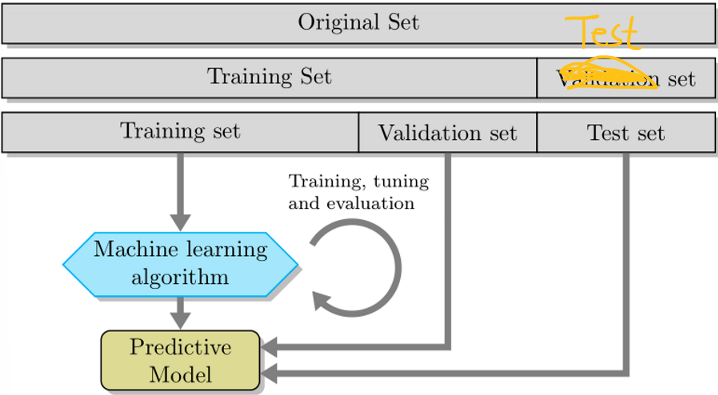
\includegraphics{./Image/Data split.png}

\subsection{Supervised vs. Unsupervised vs. Reinforced Learing}

\begin{itemize}
    \item Supervised:
          \begin{itemize}
              \item Given a set of (x,y), learn to predict y using x.
              \item Trained on a labeled dataset, which means that each input to the algorithm is
                    associated with the corresponding target or output.
              \item The goal of supervised learning is to learn a mapping from variables to the
                    corresponding output variables. The algorithm generalizes from the labeled
                    training data to make predictions or classifications on new, unseen data.
              \item Classification and regression problems fall under supervised learning. In
                    classification, the algorithm predicts the category or class of input, while
                    in regression, it predicts a continuous value.
          \end{itemize}
    \item Unsupervised:
          \begin{itemize}
              \item Given a set of x, the underlying structure of relationships of x.
              \item The algorithm explores the data's inherent structure without explicit guidance
                    on the output. (no labeled output for training)
              \item The goal of Unsupervised learning is to find patterns, relationships, or
                    structures in the data. It seeks to uncover the underlying distribution or
                    representations within the input data.
              \item Clustering and dimensionality reduction are common tasks in unsupervised
                    learning. Clustering involves grouping similar data points, while
                    dimensionality reduction aims to reduce the number of features while preserving
                    important information.
          \end{itemize}
    \item Reinforced:
          \begin{itemize}
              \item Agent interacts with an environment and learns to make decisions by receiving
                    feedback in the form of rewards or penalties.
              \item The goal is to find a policy (a strategy or decision-making process) that
                    maximizes the cumulative reward over time. The agent learns by exploring
                    different actions and overcoming the consequences of those actions.
              \item Game playing, robotic control, and autonomous systems are common applications
                    of reinforcement learning. The agent learns to take actions that lead to
                    desirable outcomes and avoid actions that lead to negative outcomes.
          \end{itemize}
\end{itemize}

\subsection{Classification vs Regression}
\begin{itemize}
    \item Classification: prediction of which class the sample belongs To
    \item Regression: Model the exact output given a sample.
\end{itemize}

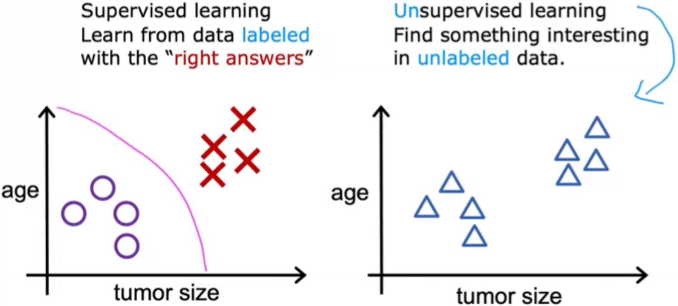
\includegraphics{./Image/Supervised vs Unsupervised.png}

\section{Linear Regression}
\subsection{Basics}
Machine learning usually has linear regression over many\-dimensions.
\[
    \hat{Y} = f_\theta(\mathsf{X})=\mathsf{X}\Theta
\]

where $\hat{\mathsf{Y}} = {(\hat{y}^{(1)},\ldots,\hat{y}^{(m)})}^T,\quad \Theta
    = {(\theta_0,\theta_1,\ldots,\theta_n)}^T$, and
\[
    \mathsf{X} =
    \begin{pmatrix}
        X^{(1)^T} \\
        \vdots    \\
        x^{(m)^T}
    \end{pmatrix}
    =
    \begin{pmatrix}
        1      & x_1^{(1)} & \cdots & x_n^{(1)} \\
        \vdots & \vdots    & \ddots & \vdots    \\
        1      & x_n^{(m)} & \cdots & x_n^{(m)}
    \end{pmatrix}
\]

Here we denote n variables $x_1,x_2,\ldots,x_n$ to represent n features
\[
    \hat{y}=f_{(\theta_0,\theta_1,\ldots,\theta_n)}(1,x_1,x_2,\ldots,x_n)=\theta_0+\theta_1x_1+\cdots+\theta_n x_n
\]

$x_0=1$ to count for the constant $\theta_0$.
\subsection{Geometry}
Data points
\{$(x_1^{(1)},\ldots,x_n^{(1)},y^{(1)}),\ldots,(x_1^{(m)},\ldots,x_n^{(m)},y^{(m)})$\}
form a (n+1) - dimensional space.

Examples for linear regression on 2-dim feature space:

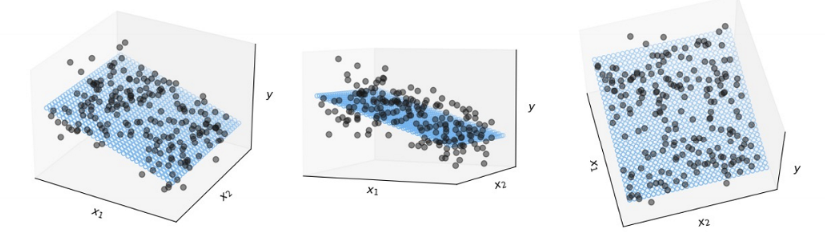
\includegraphics[scale = 0.8]{./Image/2-dim_feature_space_example.png}

\subsection{Optimizing fit}

The best fit has the smallest distance between Y and $\hat{Y} =
    f_\theta(\mathsf{X})$

We denote $J_\theta(Y,\hat{Y})$ to be the objective function (a.k.a cost or
loss function) to measure the distance between them.

Residual Sum of Squares (RSS):
\[
    J_\theta(Y,\hat{Y})   = \sum_{i=1}^{m}{(f_\theta(X^{i})-y^{(i)})}^2 = ||\hat{Y}-Y||_2^2
\]

It is a sum of the square of the difference between the data point
and the linear regression model.

To minimize the \underbar{convex} objective function, find the $\theta$ that
minimizes the loss function $J(\theta)$. It means:
\[
    J^{'}{(\theta)}=0, J^{''}(\theta)>0
\]

\subsection{Some vector and matrix calculus}
To simplify a given calculation, it is often useful to write out the
explicit formula for a single scalar element of the output in terms of nothing
but scalar variables.

\textbf{Example.} Suppose we have a column vector $\vec{y}$ of length C that is calculated by forming
the product of a matrix W that is C rows by D columns with a column vector $\vec{x}$ of length
D:

\[\vec{y}=W\vec{x}\]

Now, with some simple matrix operation, we can easily calculate the partial
derivatives of y against x. So first write out each one:

\[\vec{y}_i=\sum_{j=1}^{D}W_{i,j}\vec{x}_j\]

Write it out without the summation sign, we can overserve some tricks:

\[\vec{y}_i=W_{i,1}\vec{x}_1+W_{i,2}\vec{x}_2+W_{i,3}\vec{x}_3+\cdots+W_{i,D}\vec{x}_D\]

Since we only need the term that we are differentiating for, the rest can be
considered as constants. The derivative of a constant is zero!

\[
    \frac{\partial \vec{y}_i}{\partial \vec{x}_j} = W_{i,j}
\]

Now we can get a formula of the Jacobian matrix of the desired C x D derivative
matrix:
\[
    \begin{bmatrix}
        \frac{\partial\vec{y}_1}{\partial\vec{x}_1} & \frac{\partial\vec{y}_1}{\partial\vec{x}_2} & \cdots & \frac{\partial\vec{y}_1}{\partial\vec{x}_D} \\
        \frac{\partial\vec{y}_2}{\partial\vec{x}_1} & \frac{\partial\vec{y}_2}{\partial\vec{x}_2} & \cdots & \frac{\partial\vec{y}_2}{\partial\vec{x}_D} \\
        \vdots                                      & \vdots                                      & \ddots & \vdots                                      \\
        \frac{\partial\vec{y}_C}{\partial\vec{x}_1} & \frac{\partial\vec{y}_C}{\partial\vec{x}_2} & \cdots & \frac{\partial\vec{y}_C}{\partial\vec{x}_D}
    \end{bmatrix}
    =
    \begin{bmatrix}
        W_{1,1} & W_{1,2} & \cdots & W_{1,D} \\
        W_{2,1} & W_{2,2} & \cdots & W_{2,D} \\
        \vdots  & \vdots  & \ddots & \vdots  \\
        W_{C,1} & W_{C,2} & \cdots & W_{C,D} \\
    \end{bmatrix}
\]

So we can conclude that:
\[
    For \quad \vec{y}=W\vec{x},\quad we\quad have \quad \frac{d\vec{y}}{d\vec{x}} = W
\]

In the cases where x is a row vector:
\[
    \vec{y}=\vec{x}W\quad \implies     \frac{\partial \vec{y}_i}{\partial \vec{x}_j} = W_{j,i} \implies \frac{d\vec{y}}{d\vec{x}} = W
\]

Notice that W is the opposite of the previous example. But the idea is the
same, Jacobian matrix is similar.

Now we expand to a higher dimension. Take three dimensions as an example We
should observe that for:
\[\frac{d\vec{y}}{dW},\text{Where W is a matrix}\]

Only the partial of $\vec{y}_j$ against the jth column of W will not be zero.
The others would be zero. So we can write:
\[\frac{\partial\vec{y}_j}{\partial W_{i,j}}=\vec{x}_i\]

Let F represent the 3d array representing the derivative of $\vec{y}$ against
W:
\[
    F_{i,j,k}= \frac{\partial\vec{y}_i}{\partial W_{j,k}}\text{, then } F_{i,j,i}=\vec{x}_j\text{, and all other entries are zero.}
\]

So now we can define a new \textit{two-dimensional} array G as:
\[G_{i,j}=F_{i,j,i}\]

Now onto multiple samples:

For example, let X be a two-dimensional array with N rows and D columns, and W
the same as previous, D rows and C columns.
\[Y=XW \implies Y_{i,j}=\sum_{k=1}^{D}X_{i,k}W_{k,j}\text{ , and the partial is:} \frac{\partial Y_{a,b}}{\partial X_{c,d}}\]

Same idea as before: nonzero exists only when a = c. So:
\[
    \frac{\partial Y_{i,j}}{\partial X_{i,k}} = W_{k,j}
\]

We have now generalized the matrix derivative.

The last topic is the chain rule:

\[
    \vec{y}=VW\vec{x}\text{, define }\vec{m}=W\vec{x}\text{, then }\vec{y}=V\vec{m}.\quad \implies \frac{d\vec{y}}{d\vec{x}}= \frac{d\vec{y}}{d\vec{m}}\frac{d\vec{m}}{d\vec{x}}
\]

In machine learning, the loss function that is generally optimized is a scalar
function such as $x\rightarrow y \rightarrow $ dependencies of z. So we can
write:

\[\frac{\partial z}{\partial x} = {(\frac{\partial y}{\partial x})}^T \frac{\partial z}{\partial y}\]

\subsection{ChatGPT teaching time}

\textbf{Step 1: Prepare the Data}

You should have a set of data points in the form of pairs $(x_1, y_1), (x_2,
    y_2), \ldots, (x_n, y_n)$, where $x_i$ is the independent variable, and $y_i$
is the dependent variable.

\textbf{Step 2: Create the Design Matrix $X$}

The design matrix $X$ is a matrix of size $n \times (d+1)$, where $n$ is the
number of data points and $d$ is the degree of the polynomial you want to fit
(e.g., $d=2$ for quadratic regression).

For quadratic regression ($d=2$), $X$ looks like this:

\[
    X = \begin{bmatrix}
        1      & x_1    & x_1^2  \\
        1      & x_2    & x_2^2  \\
        \vdots & \vdots & \vdots \\
        1      & x_n    & x_n^2  \\
    \end{bmatrix}
\]

Each row corresponds to a data point, and each column represents a term in the
polynomial equation. The first column contains $1$s for the intercept term, the
second column contains the $x$ values, and the third column contains the $x^2$
values.

\textbf{Step 3: Create the Coefficient Vector $b$}

The coefficient vector $b$ contains the coefficients of the polynomial terms.
For quadratic regression ($d=2$), $b$ is a vector of size $d+1 = 3$:

\[
    b = \begin{bmatrix}
        b_0 \\
        b_1 \\
        b_2 \\
    \end{bmatrix}
\]

\textbf{Step 4: Create the Observation Vector $Y$}

The observation vector $Y$ contains the dependent variable values for each data
point. It's a vector of size $n$:

\[
    Y = \begin{bmatrix}
        y_1    \\
        y_2    \\
        \vdots \\
        y_n    \\
    \end{bmatrix}
\]

\textbf{Step 5: Solve for $b$ Using Matrix Operations}

The goal is to find the coefficients $b$ that minimize the error in the
polynomial regression equation. This can be done by solving the linear system
of equations:

\[
    Xb = Y
\]

This is a system of $n$ equations (one for each data point) and $d+1$ unknowns
(the coefficients $b_0, b_1, \ldots, b_d$).

To solve for $b$, you can use matrix operations. Specifically, you can use the
equation:

\[
    b = (X^TX)^{-1}X^TY
\]

Here's what each part of the equation does:

- $X^T$ is the transpose of matrix $X$. It converts the $n \times (d+1)$ matrix into a $(d+1) \times n$ matrix.
- $X^TX$ is the matrix multiplication of the transposed matrix $X^T$ and $X$, resulting in a $(d+1) \times (d+1)$ matrix.
- $(X^TX)^{-1}$ is the inverse of the $(d+1) \times (d+1)$ matrix.
- $X^TY$ is the matrix multiplication of the transposed matrix $X^T$ and vector $Y$, resulting in a $(d+1) \times 1$ vector.
- $b$ is the coefficient vector you want to find.

Once you calculate $b$, it contains the coefficients of the polynomial equation
that best fits your data.

\textbf{Step 6: Use the Polynomial Equation}

With the coefficients $b$ obtained, you can construct the polynomial equation:

\[
    y = b_0 + b_1x + b_2x^2
\]

This is the equation of the polynomial regression model.

This explanation covers quadratic regression ($d=2$), but you can extend the
same principles to higher-degree polynomial regressions by increasing the
number of columns in the design matrix $X$ and the size of the coefficient
vector $b$.

\subsection{Metrics and prediction errors}

Denote total samples as N, true label as Y, prediction as $\hat{Y}$, the
average of testing set as $\bar{Y}$

\begin{itemize}
    \item Mean Absolute Error (MAE): MAE = $\frac{1}{N}\sum_{n}^{N}|Y_n-\hat{Y}_n|$
    \item Mean Square Error (MSE): MSE = $\frac{1}{N}\sum_{n}^{N}(Y_n-\hat{Y}_n)^2$
    \item Root Mean Square (RMSE): RMSE = $\sqrt{MSE}$
    \item R-square: $R^2 = 1 - \frac{\sum{(Y-\hat{Y})^2}}{\sum{(Y-\bar{Y})^2}}$
\end{itemize}

The higher the R-square, the more testing data points are from the prediction
regression line.

\section{Regression with Shrinkage and Logistic Regression}

\subsection{Bias and Variance}

\includegraphics*[scale = 0.9]{./Image/Bias_Variance.png}

Bias = $\theta - \mathbb{E}\hat{\theta}$ and Variance =
$\mathbb{E}(\hat{\theta} - \mathbb{E}\hat{\theta})^2$

\begin{itemize}
    \item $\hat{\theta}$ is an estimation from the sample
    \item $\mathbb{E}$ is the expectation w.r.t.samples (i.e., avg estimator)
    \item We can only directly compute $\hat{\theta}$ from the observed samples. We do
          not know $\theta$
\end{itemize}

Def: The expectation $\mathbb{E}$ is used to find the average or expected
behavior of random variables.

\subsection{Expected prediction error (Risk)}

\begin{itemize}
    \item The relation of input and output is modeled by the function $f$.
    \item Due to the noise from observation, y = $f(X) + \epsilon$, where
          $\mathbb{E}(\epsilon)=0$ and Var$(\epsilon)={\epsilon}^2$
    \item For any fixed input $X$ and its label $y$, the expected prediction error (EPE)
          on $X$ is:
\end{itemize}

\[
    EPE(X)=\mathbb{E}[(y-\hat{f}(X))^2]=Bias(\hat{f}(X))^2+Var(\hat{f}(X))+\epsilon^2
\]
where
\[
    Bias(\hat{f}(X)) = f(X)-\mathbb{E}[\hat{f}(X)]
\]

\[
    Var(\hat{f}(X))=\mathbb{E}[(\hat{f}(X)-\mathbb{E}[\hat{f}(X)]^2)]
\]

Becuase Risk = Bias$^2$+Variance:
\[
    \mathbb{E}[(y-\hat{f}(X))^2]=Bias(\hat{f}(X))^2+Var(\hat{f}(X))=(y-\mathbb{E}\hat{f}(X))
\]

In general, low variance will cause high bias and vice versa. So we have to
make trade-offs.

For example: if we repeatedly train the sample data for too long.
\begin{itemize}
    \item It may perfectly fit the training data. So low bias and high variance since
          the model will vary significantly among different training data.
    \item If the model is constant among different training data, the prediction
          variance is zero but definitely the prediction bias is very high.
\end{itemize}

\subsection{Bias-variance trade-off}

\includegraphics*{./Image/Bias-variance trade-off.png}

The complex model will lead to high bias, hence \textbf{Overfitting}

A simple model will lead to high variance, hence \textbf{Underfitting}

A good fit will have the lowest EPE\(X\)

\subsection{Shrinkage methods}
Ordinary least squares are prone to learn a low bias high variance model.

Tunning model complexity is a way to sacrifice some bias to reduce the variance
to achieve lower EPE.

Coding examples of the methods used can be found
\href{https://colab.research.google.com/drive/1ENbxMw0y86eHTorCbd1riAVOQU25-GEO?usp=sharing}{here}.
\begin{itemize}
    \item Ridge regression adds a regularization term to the linear regression cost
          function to address the problem of multicollinearity and overfitting.

          Recall the linear function $\hat{Y}=\mathsf{X}\Theta+\theta_0$ Where we sperate
          the constant term from X and $\Theta$.

          Now the ordinary least squares can be expressed as:

          \[
              \hat{\Theta}=\text{argmin}_\Theta||\mathsf{X}\Theta+\theta_0-Y||_2^2
          \]

          Here argmin is the symbol to indicate the input that could minimize the
          smallest out, which is to minimize the L2 norm.

          Ridge regression aims to shrink the parameter by imposing a penalty on the square of
          the magnitude of the coefficients:
          \[
              \hat{\Theta}_{rigid}=\text{argmin}_\Theta||\mathsf{X}\Theta+\theta_0-Y||_2^2 + \lambda||\Theta||_2^2
          \]

          The penalty term is $||\Theta||_2^2=\sum_{i=1}^{n}=\theta_i^2$ (a.k.a. L2 Norm)

          Note that the bias term $\theta_0$ is not included in the penalty term.
          $\lambda$ is a hand-crafted hyper-parameter.

          Notes on the penalty term
          \begin{itemize}
              \item When there are many correlated features in a linear regression model, their
                    coefficients can become poorly determined and exhibit high variance.
              \item A wildly large positive coefficient on one variable can be canceled by a
                    similarly large negative coefficient on its correlated cousin.
              \item The penalty term regularizes the coefficients such that if the coefficients
                    take large values, the optimization function is penalized. Therefore, the above
                    problem is alleviated.
          \end{itemize}

    \item Lasso regression: Linear regression technique that combines the principles of
          linear regression with L1 regularization.
          \[
              \hat{\Theta}_{rigid}=argmin_\Theta||\mathsf{X}\Theta+\theta_0-Y||_2^2 + \lambda||\Theta||_1
          \]

          The penalty term is $\lambda||\Theta||_1=\sum_{i=1}^{n}|\theta_i| $(a.k.a. L1
          Norm), which is designed for measuring the sparsity of parameters.

          Sparsity implies the number of zeros in $\Theta$. If many elements in it are
          around zero, fewer features will be used, namely, the model complexity is
          reduced.

    \item In comparison:

          Ridge regression's penalty term regularizes the coefficients such that the
          coefficients won't be large.

          Lasso regression's penalty term regularizes the coefficients such that
          coefficients are sparse (containing many zeros elements).
\end{itemize}

\section{Classification}

Classification is a process related to categorization, in which ideas and
objects are recognized, differentiated and understood.

Binary classification:
\begin{itemize}
    \item True or false about a statement
    \item For example: is it a cat? (0 for no and 1 for yes)
\end{itemize}

Multi-class classificaiton:
\begin{itemize}
    \item More than two categories, usually use 0, 1, 2, 3, \ldots to label categories
    \item For example, which animal is in the photo? Cat/dog/pig/duck/\ldots.
\end{itemize}

We use \textbf{decision boundary} to partition the entire feature space into
multiple parts. One for each category.

A linear classifier is a linear model we use to classify data based on a linear
combination of input features. We usually learn some function to divide.

\subsection{Logistic regression for classificaiton}

Logistic regression models the probabilities for classification problems for an
even occurring.

The cut-off rule is a transformation that maps linear functions' range
($-\infty,+\infty$) to the range of probability (0,1). In the equation, it
refers to z and p.

Then we see a dramatic rise in the boundary value (which is zero) as shown
below:

\includegraphics*{./Image/Basic Sigmoid Funciton.png}

logit:
\[
    z=\text{logit}(p)=\ln\frac{p}{1-p}
\]
\[
    -z=\ln\frac{1-p}{p}\implies e^{-z}=\frac{1}{p}-1
\]

sigmoid:
\[
    \text{logit}^{-1}(z)=p=\frac{1}{1+e^{-z}}
\]

The following is a probability view of logit:
\begin{itemize}
    \item Event A and its probability to happen: $P(A)=p$, $P(A^C)=1-p$
    \item The odds of an event is the ratio of the probability of an event to the
          probability of its complement. So we can express the following:
          \[
              \text{odds}(p)=\frac{p}{1-p}
          \]
    \item The range of odds is (0,$+\infty$). Logit is defined as log-odds with range
          ($-\infty,+\infty$).
    \item Recall the linear regression function:
          \[
              f_{\Theta}=X^T\Theta\in(-\infty,+\infty)
          \]
    \item Recall our goal is to find $(P(y=1|X))$. We should have
          \[
              P(\hat{y}=1|X)=\text{logit}^{-1}(X^T\Theta)=\frac{1}{1+e^{-(X^T\Theta)}}    \in(0,1)
          \]
    \item  The equation above is the basic formulation of logistic regression.
    \item Classification rule:
          \[
              P(\hat{y}=1|X) \ge0.5 \implies \hat{y}=1,\text{ otherwise } \hat{y}=0
          \]
    \item Like linear regression, $\Theta$ is the learnable parameter.
    \item LR is more robust to outliers
\end{itemize}

Sometimes, we denote $\text{logit}^{-1}()$ as sigmoid$()$ or $\sigma()$.

As mentioned, it rises dramatically to 0. Also we know $\sigma(X^T\Theta)\ge
    0.5 \iff X^T\Theta\ge0.$
\begin{align*}
    X^T\Theta\ge 0 & \implies \hat{y}=1 \\
    X^T\Theta\le 0 & \implies \hat{y}=0
\end{align*}

The decision boundary is the hyperplane $z=X^T\Theta$

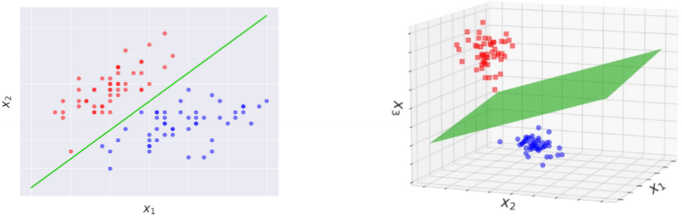
\includegraphics{./Image/Boundary Hyperplane.png}

\subsection{Supervision criteria}

For each sample $X^{(i)}=({x_1^{(i)},\ldots,x_n^{(i)}})$ we have:
\[
    P(\hat{y}^{(i)}=1|X^{(i)})=\sigma(X^{(i)T}\Theta)=\frac{1}{1+e^{-(X^{(i)T}\Theta)}}\in(0,1)
\]
which is a function with respect to $\Theta$.

\begin{itemize}
    \item if $y^{(i)}=1$, we expect $P(\hat{y}^{i}=1|X^{(i)})$ approaches 1 as close as
          possible.
    \item if $y^{(i)}=0$, we expect
          $P(\hat{y}^{i}=0|X^{(i)})=1-P(\hat{y}^{(i)}=1|X^{(i)})$ approaches 0 as close
          as possible.
\end{itemize}

To generalize, we can write the probability that the label is correctly
predicted as
\[
    p_i\equiv P(\hat{y}^{(i)}=1|X^{(i)})^{y(i)}(1-P(\hat{y}^{(i)}=1|X^{(i)}))^{1-y(i)}
\]

Namely:
\begin{itemize}
    \item When $y^{(i)}=0\quad \implies \quad P(\hat{y}^{i}=0|X^{(i)})$
    \item When $y^{(i)}=1\quad \implies \quad P(\hat{y}^{i}=1|X^{(i)})$
    \item So no matter which category the sample belongs to, $p_i$ can represent
          the probability that the prediction $\hat{y}^{(i)}$ matches the true label
          $y^{(i)}$
\end{itemize}

Next, we consider the joint probability for all the training samples, and
maximize it to learn $\Theta$.

Since the samples are independent of each other, the joint probability can be
written as:

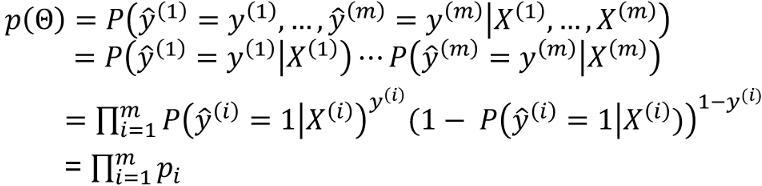
\includegraphics[scale = 0.9]{./Image/Joint probability of supervision critiria.png}

We want to make $p(\Theta)$ as large as possible. Maximizing a likelihood
function is called \textit{maximum likelihood estimation (MLE)}.

\subsection{Cross-entropy}
Binary cross-entropy error $\equiv
    -y\text{ln}P(y)-(1-y)\text{ln}(1-P(y)),y\in\{0,1\}$ It is a concept from
information theory. $P(y)$ is the probability density function of taking value
y. In our case:
\[
    P(y)=P(\hat{y}^{(i)}=1|X^{(i)})=\frac{1}{1+e^{- X^{(i)T}\Theta}}
\]

\begin{itemize}
    \item when y = 1, error = -ln$(\frac{1}{1+e^{-\Theta X^{(i)T}}})$
    \item when y = 0, error = -ln$(1-\frac{1}{1+e^{-\Theta X^{(i)T}}})$
\end{itemize}

Cross-entropy can be plotted as follows. To minimize it, we find the
interception.

\includegraphics*{./Image/cross entropy.png}

Similar to RSS, we could minimize cross-entropy through $\frac{\partial
        \mathbb{E}(\Theta)}{\partial \Theta}|\Theta^*=0$ However, it will be too
difficult. So we try \textbf{gradient descent}.

For a twice differentiable function (so that a second derivative exists)
$f:\mathbb{R}^n\rightarrow\mathbb{R}$, the gradient $\nabla f(\Theta)$ points
in the direction of the steepest ascent or descent at $\Theta$.
\[
    \nabla f(\Theta)=\frac{\partial f(\Theta)}{\partial \Theta} = (\frac{\partial f(\Theta)}{\partial \theta_1}, \ldots, \frac{\partial f(\Theta)}{\partial \theta_n})   \text{ , where }\Theta = \{\theta_1,\ldots,\theta_n\}
\]

Gradient descent is designed to update parameters in the \textbf{opposite}
the direction of the gradient. Through iterative updates, an optimal solution for
our goal of min$f(\Theta)$ can be attained. The simple algorithm can be
illustrated below:

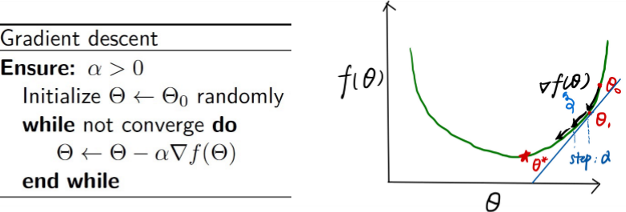
\includegraphics{Image/Gradient descent.png}

\begin{itemize}
    \item $\alpha$ is a small enough hyper-parameter called learning rate.
    \item Too small will lead to a very slow learning process.
    \item Too large leads to bad convergence. (Might diverge)
    \item You might be able to change it at every iteration
\end{itemize}

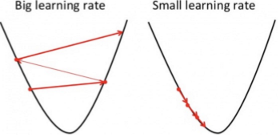
\includegraphics{./Image/learning rate for gradient descent.png}

\subsection{ChatGPT example of gradient descent}

The linear model is defined as:
\[ f_\Theta(x_1, x_2) = \theta_0 + \theta_1 x_1 + \theta_2 x_2 \]

The Mean Squared Error (MSE) loss is given by:
\[ \mathcal{L}(\Theta) = \frac{1}{2N} \sum_{i=1}^{N} (f_\Theta(x_1^{(i)}, x_2^{(i)}) - y^{(i)})^2 \]

The gradient descent update rule for the parameters is:
\[ \theta_j \leftarrow \theta_j - \alpha \frac{\partial}{\partial \theta_j} \mathcal{L}(\Theta) \]

Partial Derivatives:
\begin{align*}
    \frac{\partial}{\partial \theta_0} \mathcal{L}(\Theta) & = \frac{1}{N} \sum_{i=1}^{N} (\hat{y}^{(i)} - y^{(i)})                 \\
    \frac{\partial}{\partial \theta_1} \mathcal{L}(\Theta) & = \frac{1}{N} \sum_{i=1}^{N} (\hat{y}^{(i)} - y^{(i)}) \cdot x_1^{(i)} \\
    \frac{\partial}{\partial \theta_2} \mathcal{L}(\Theta) & = \frac{1}{N} \sum_{i=1}^{N} (\hat{y}^{(i)} - y^{(i)}) \cdot x_2^{(i)}
\end{align*}

Finally, the updated equations for each parameter are:
\begin{align*}
    \theta_0 & \leftarrow \theta_0 - \alpha \frac{\partial}{\partial \theta_0} \mathcal{L}(\Theta) \\
    \theta_1 & \leftarrow \theta_1 - \alpha \frac{\partial}{\partial \theta_1} \mathcal{L}(\Theta) \\
    \theta_2 & \leftarrow \theta_2 - \alpha \frac{\partial}{\partial \theta_2} \mathcal{L}(\Theta)
\end{align*}

For complex and nonconvex functions, gradient descent usually falls into a
local minimum instead of the global minimum.

\section{Model Evaluation and Trainning}

\subsection{Multi-class Classification}

Extend the previous binary regression methods to more than 2 classes.

Multinomial logistic regression extends the logistic regression model to K$\ge$
2 using \textit{one-versus-all}

\includegraphics*{Image/Multinomial logistic regression.png}

Each $\Theta_k$ represents a line that separates one type from the rest. So we
need a total of k-1 $\Theta$ since the last one is redundant.\ k=0 means it does
not belong to anything. So $\Theta_0$ is all zeros by definition.

\subsection{Discriminative and Generative Clssifier}

\begin{itemize}
    \item Generative models model both the input X and the output Y. ($P(y=k, X;\Theta)$)
          Bayes classifier is a good example. The theorem of minimizing risk R(h) is

          \[
              h^* = (P(Y=1|X)>0.5) \quad 1 : 0
          \]

    \item Discriminative models model only the output Y given X. ($P(y=k|X;\Theta)$)
          Logistic regression is a discriminative model because we do not have a model
          for the input X. We only model the conditional probability $P(Y|X)$
\end{itemize}

\subsection{Mertics for Classification}

Metrics to evaluate model performance, we count the number of occurrences for the
following.

\begin{itemize}
    \item TP is ``true positive'': predict correctly as positive
    \item FP is ``false positive'': predict incorrectly as positive
    \item TN is ``true negative'': predict correctly as negative
    \item FN is ``false negative'': predict incorrectly as negative
\end{itemize}

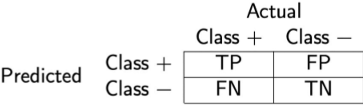
\includegraphics{Image/Metrics to evaluate models.png}

Accuracy = frcation of correct predictions = $\frac{TP+TN}{TP+FP+TN+FN}$

Precision = accuracy of the positive predictions = $\frac{TP}{TP+FP}$

Recall (a.k.a. sensitivity) = accuracy of positive class = $\frac{TP}{TP+FN}$

F1 score is calculated from precision and recall and is the \textbf{harmonic
    mean} of them. The highest possible value is 1.0
\[
    F_1=2\frac{\text{precision}\times\text{recall}}{\text{precision}+\text{recall}}  = \frac{TP}{TP+0.5(FP+FN)}
\]

\subsection{Confusion matrix}
Confusion matrix is a specific table layout that allows visualization of the
performance.

A matrix is a square with a side length equal to the total categories. One side is
the actual class and one side is the prediction. The Diagonal represents the correct
prediction whereas the other cells represent a false prediction to a different
class.

Following are the examples of 2 classes and 10 classes:

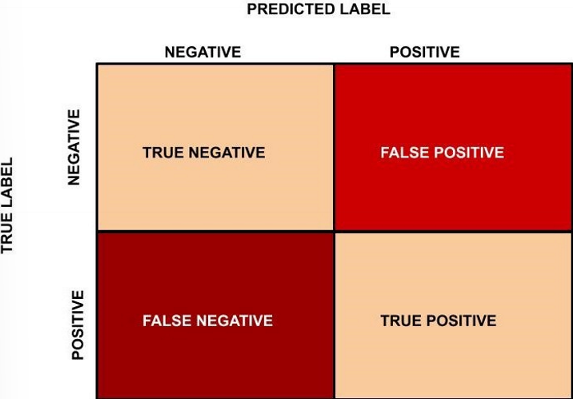
\includegraphics{./Image/Confusion matrix 2 class.png}

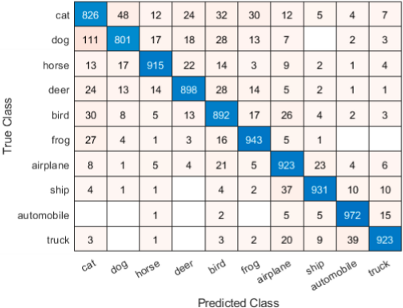
\includegraphics{./Image/Confusion matrix.png}

\subsection{Receiver operating characteristic curve (ROC)}

ROC is a graphical plot that illustrates the diagnostic ability of a binary
classifier system as its discrimination threshold is varied.

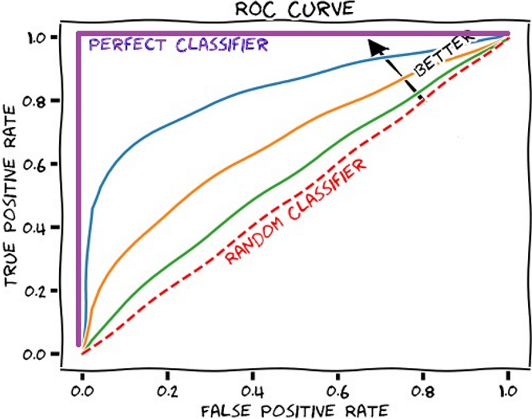
\includegraphics{./Image/ROC curve.png}

For random guess, true positive rate (TPR) = false positive rate (FPR). In
contrast, perfect classifiers have only TPR and no FPR. So as long as the graph
is above the random guess line (towards the perfect classifier), it is better than
a random guess.

Comparing between the lines can be done by calculating the area under the curve
if not easily visualized.

Refer to the slide for how it is calculated.

\subsection{Cross validation}
Performing machine learning involves creating a model, which is trained on a
training data set and then process the test data set.

We sometimes also use a validation data set, which is a data set of examples
used to tune the hyperparameters of the model.

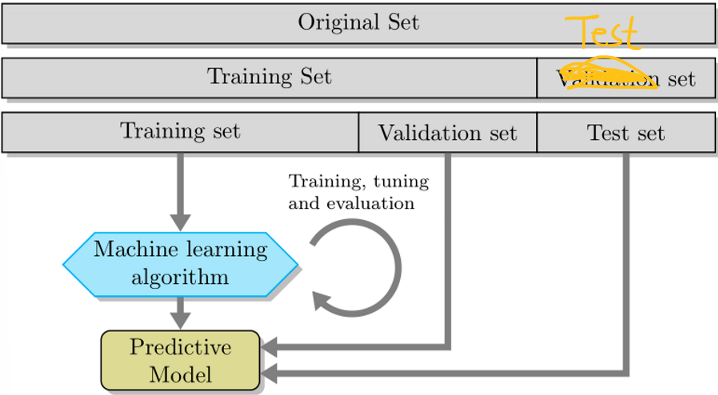
\includegraphics{./Image/Data split.png}

Cross-validation is used to evaluate AI models on a small-scale data set.
\begin{itemize}
    \item Shuffle the data set randomly and split the data set into k groups.
    \item For each unique group:
          \begin{itemize}
              \item Take the group as a holdout or test data set.
              \item Take the remaining groups as a training data set.
          \end{itemize}
    \item Summarize the skill of the model using all the model evaluation scores.
\end{itemize}

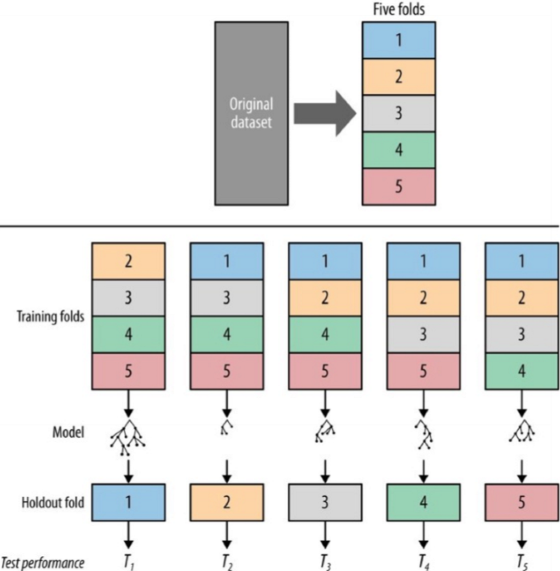
\includegraphics{./Image/K group cross validation.png}

Leave-One-Out Cross-Validation: basically a special K group case where each
group only contains one set of data.

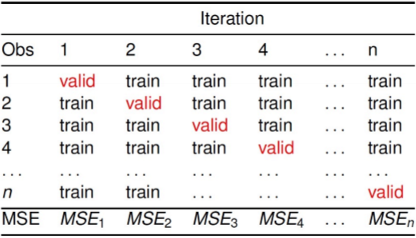
\includegraphics{./Image/Leave-Out-Out Cross_Validation.png}

LOOCV estimate (with n samples) of test error is given by
\[
    CV_{(n)}=\frac{1}{n} \sum_{i=1}^{n}MSR_i
\]
which is a single number, with no randomness. (K-fold has randomness since the
the split group has different ways of formation.)

K-fold have each group formed randomly with a size larger than 1. Potentially
faster approach.

\begin{itemize}
    \item Randomly divide the data set into k folds.
    \item For $b = 1,\ldots,k:$
          \begin{itemize}
              \item Use $b$th fold as a validation set.
              \item Use the rest as the training set.
              \item Compute validation error on $b$th fold.
          \end{itemize}
    \item Estimate test error using:
          \[
              CV_{(k)}=\sum_{b=1}^{k}\frac{n_b}{n}MSE_b
          \]
          where $n_b$ is the total number obervations in $b$th fold and $n$ is the total
          number of samples.
\end{itemize}
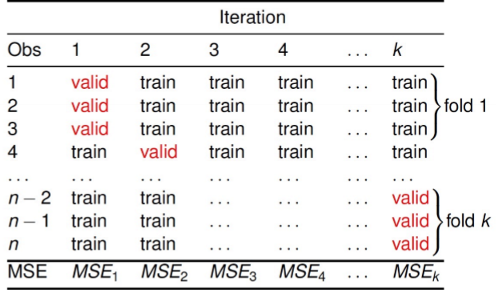
\includegraphics{./Image/K fold Cross-Validation.png}

\section{Bayesian Classifier}
\subsection{Basic probabilities}
Chain rule:
\[
    P(x,y,z) = p(x)p(y|x)p(z|x,y) = p(z)p(y|z)p(x|y,z)
\]
Conditional Probability:
\[
    P(X=x|Y=y)=\frac{P(X=x)\cap P(Y=y)}{P(Y=y)}
\]
\[
    P(x|y)=\frac{p(x,y)}{p(y)}
\]

Marginalization:
\[
    p(x)=\sum_{y}P(x,y)=\sum_{y}P(y)P(x|y)
\]
Bayes Rule:
\[
    P(x|y)=\frac{P(x)P(y|x)}{P(y)}
\]
\[
    P(x|y,z)=\frac{P(x|z)P(y|x,z)}{P(y|z)}
\]
\subsection{Defination:}

Bayes' Original Theorem and Marginal Probability:
\[
    p(B|A)=\frac{p(A|B)p(B)}{p(A)}    \quad p(A)=\sum_{B_i,\in S_B}p(A|B_i)p(B_i)
\]

Probability of $A$ is the sum of all probabilities of $A$ given $B_i$ for all
$B$

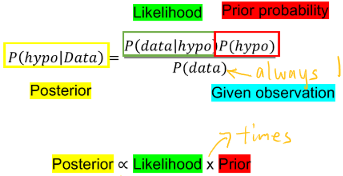
\includegraphics{./Image/Bayesian.png}

Let $A_1, A_2, \ldots, A_k$ be the attributes with discrete values in class C.
Given a test example, d with observed attribute values $a_1, a_2, \ldots, a_k$

If we assume that all attributes are conditionally independent, then we can say
that:
\[
    Pr(A_1=a_1, A_2=a_2,\ldots,A_k=a_k)Pr(C=c_j)=\prod_{i=1}^{k}Pr(A_i=a_i|C=c_j)
\]

Final Bayesian classifier:

\[
    Pr((C=c_j)| (A_1=a_1, A_2=a_2,\ldots,A_k=a_k)) = \frac{Pr(C=c_j)\prod_{i=1}^{k}Pr(A_i=a_i|C=c_j)}{\sum_{r=1}^{k}(Pr(C=c_r)\prod_{i=1}^{k}Pr(A_i=a_i|C=c_j))}
\]

However, if we only need a decision on the most probable class for the test
instance, we only need the numerator as its denominator is the same for every
class.

Just need to find the $c_j$ with the maximum value of the following:

\[
    c = \prod_{i=1}^{k}P(A_i=a_i|C=c_j)P(c_j)
\]

\begin{itemize}
    \item Bayesian learning is usually quite accurate with a certain degree of violation
          in practice.
    \item If the model is more mixed, it will tend to be more accurate.
    \item This approach is very efficient.
\end{itemize}

\subsection{Example question:}

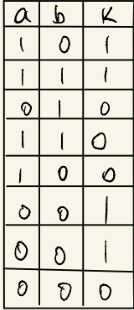
\includegraphics{./Image/Bayesian example.png}
Assume fearture $a,b$ are independent, find the prediction probability for $P(k=0|a=1,b=1)$

\[
    P(k=0|a=1,b=1)=\frac{P(k=0,a=1,b=1)}{P(a=1,b=1)}
\]
Here $P(k=0,a=1,b=1)=P(k=0)P(a=1|k=0)P(b=1|k=0)=\frac{1}{2} \times \frac{1}{2}
    \times \frac{1}{2}$

Then calculate the denominator:
\begin{itemize}
    \item Proper way:

          $P(a=1,b=1)=\sum_{i}^{\text{all possible k}}P(k=i|a=1,b=1)$

          $=P(k=0|a=1,b=1)+P(k=1|a=1,b=1)$

          where $P(k=1|a=1,b=1)=P(k=1)P(a=1|k=1)P(b=1|k=1)=\frac{1}{2} \times \frac{1}{2}
              \times \frac{1}{4}$

          So we have $P(a=1,b=1)=\frac{1}{8}+\frac{1}{16}=\frac{3}{16}$

    \item Sneaky way: Since a and ba are independent.
          \[
              P(a=1,b=1)=P(a=1\land b=1)=P(a=1)\times P(b=1) = \frac{4}{8} \times \frac{3}{8} =\frac{3}{16}
          \]
\end{itemize}

So the answer is $\frac{\frac{1}{8}}{\frac{3}{16}}=\frac{2}{3}$

\section{Support vector machines (SVM)}
SVMs are \textbf{linear classifiers} that find a hyperplane to separate two
class of data, positive and negative.

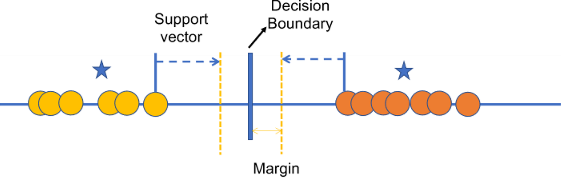
\includegraphics{./Image/SVM toy example.png}

Support vectors are data points that are closer to the hyperplane and influence
the position and orientation of the hyperplane.

\subsection{Basic concepts}

Let the set of training examples D be represented by:
$\{(\vec{x}_1,y_1),(\vec{x}_2,y_2),\ldots,(\vec{x}_r,y_r)\}$, where
$x_i=(x_1,x_2,x_3,x_4,\ldots,x_n)$.

So we have r samples each with n features. Then $x_i$ is an input vector in a
real-valued space $X\in R^n$ and $y_i$ is its class label (output value),
$y_i\in\{1,-1\}$. 1 for the positive class and -1 for the negative class.

SVM finds a linear function of the form (w: weight vector)
\[
    f(x)=<w \cdot x>+b
\]

\begin{align*}
    y_i & = 1  & \text{if }<w\cdot x_i> + b \ge 0 \\
    y_i & = -1 & \text{if } <w\cdot x_i> + b < 0
\end{align*}

Then the hyperplane that separates positive and negative training data is
$<w\cdot x> + b = 0$. It is also called the \textbf{decision boundary
    (surface)}

A robust separating hyperplane has a ``fat'' margin (far from both sides of
examples). So the goal is to find the fattest separating hyperplane.

\subsection{linarly separable SVM}
Assume that the data are linearly separable.

Consider a positive data point $(x^+,1)$ and a negative $(x^-,-1)$ that are
closest to the hyperplane.

We define two parallel hyperplanes, $H_+, H_-$ that pass through $x^+,x^-$
respectively. The two hyperplanes should also be parallel to the decision
boundary:
\[
    w^T x+b=<w\cdot x>+b=0
\]

We should be able to get:

\begin{align*}
    H_+: \quad <w\cdot x>+b & =1                           \\
    H_-: \quad <w\cdot x>+b & =-1                          \\
    \text{such that}                                       \\
    <w\cdot x_i>+b          & \ge 1 \quad \text{if }y_i=1  \\
    <w\cdot x_i>+b          & \le 1 \quad \text{if }y_i=-1
\end{align*}

Support vectors are the data points that lie closest to the decision boundary
(hyperplane).

So at a Support Vector $(x_s,y_s)$, we have $y_s(w^T x_s+b)=\pm 1$

\includegraphics*{./Image/Support vector.png}

\subsection{Compute the margin}
To compute the distance between the two Marigin hyperplanes $H_+$ and $H_-$,
recall that the (perpendicular) distance from a point $x_i$ to the hyperplane
$<w\cdot x>+b=0 $ is:
\[
    \frac{|<w\cdot x_i>+b|}{||w||}
\]

Given $||w||=\sqrt{<w\cdot w>}=\sqrt{w_1^2+w_2^2+\cdots+w_n^2}$

So for all support vectors on hyperplane, their distance is $\frac{y_i(w^T x_i
        +b)}{||w||}\to \frac{1}{||w||}\implies $ the summarized distance is called the
margin $\gamma = \frac{2}{||w||}$

So now, our aim is basically to maximize the margin, which is to minimize the
norm of w.

\subsection{Optimization of SVM}

Transforming the objective:
\[
    \max_w\frac{2}{||w||}\to \min_w \frac{1}{2}||w|| \to \min_w \frac{1}{2}||w||^2
\]

So we need $\min_w \frac{1}{2}||w||^2$ s.t. $y_i(w^T x_i +b)\ge 1$ or $g_i
    (w,b) = 1 - y_i (w^R x_i +b)\le 0; i = 1,2,\ldots , m$

Use Lagrange multipliers to solve the problem, write down the loss function as:
\begin{align*}
    L(w,b,\alpha) & = \frac{1}{2}||w||^2 + \sum_{i=1}^{m}\alpha_i (1 - y_i (w^R x_i +b)) \\
    \alpha        & = (\alpha_1;\alpha_2;\ldots;\alpha_m)
\end{align*}

Optimization theory says that an optimal solution to the Lagrangian method must
satisfy Karush-Kuhn-Tucker (KKT) conditions, which are \textbf{necessary but
    not sufficient}

\includegraphics*{./Image/KKT conditions.png}

Now take the derivative with respect to w and b, and set them equal to zero:
\begin{align*}
    L(w,b,\alpha)                          & = \frac{1}{2}||w||^2 + \sum_{i=1}^{m}\alpha_i (1 - y_i (w^R x_i +b)) \\
    \frac{\partial L}{\partial w} = 0      & \implies w = \sum_{i=1}^{m}\alpha_i y_i x_i                          \\
    \frac{\partial L}{\partial \alpha} = 0 & \implies 0 = \sum_{i=1}^{m} \alpha_i y_i
\end{align*}

Now establish the KKT condition:
\begin{align*}
    \alpha_i                     & \ge 0 \\
    y_i(w^T x_i +b)-1            & \ge 0 \\
    \alpha_i (y_i(w^T x_i +b)-1) & =0
\end{align*}
Note that $\alpha_i = 0$ or $(w^T x_i +b)-1 = 0$ for the third condition.
\begin{itemize}
    \item If $(w^T x_i +b)-1 = 0$, it means that the sample point $(x_i,y_i)$ is a
          support vector, and $\alpha_i>0$
    \item if $(w^T x_i +b)-1 > 0$, it means that the distance between the sample point
          $(x_i,y)$ is farther than support vectors, and $\alpha_i = 0$
\end{itemize}

Now the optimization problem is a quadratic programming (QP) problem. There are
some effective algorithm to solve the problem.

If we find the optimal $\alpha$, we can find w using $w =
    \sum_{i=1}^{m}\alpha_i y_i x_i$.

For the optimal b, since we have optimal w and $y_s(w^T x_s+b)=1$, we can use
arbitrary support vector $x_s,y_s$ to get $b=(\frac{1}{y_s}-w^T x_s)$, where
$S=\{ \alpha_i>0, i = 1,2,\ldots,m\}$ are the indices of support vector.

Practically, we suggest averaging over all eligible support vectors to
alleviate numerical error:
\[
    b = \frac{1}{|S|}\sum_{s\in S}    (\frac{1}{y_s}-w^T x_s)
\]

\subsection{Soft-margin SVM}

Linear separable case is the ideal situation, real-life data may have noise or
errors which would not satisfy the constraints, thus, no solution!

So the idea of soft-margin SVM is to allow some noisy samples not to obey the
condition:
\begin{align*}
    \text{goal:}  \min            & \frac{1}{2}||w||^2               \\
    \text{s.t. }y_i(w^T x_i + b)  & \ge 1 \text{ for clean } i       \\
    \text{and }  y_i(w^T x_i + b) & \ge -\infty \text{ for noisy } i
\end{align*}
\subsubsection{Penalty function}
To minimize the number of noisy samples, we can use a new \textbf{penalty} item and our objective is transformed to:
\[
    \min_{w,b}\frac{1}{2}||W||^2+C\sum_{i=1}^{m}l_{0/1}(y_i(w^T x_i+b)-1)
\]

Here, C is a constant and $l_{0/1}(z)=1$ if $z<0$, otherwise, it is 0. $z =
    (y_i(w^T x_i+b)-1) $ in the equation.

So if the sample is in the constraint condition, there is no penalty.
Otherwise, $l_{0/1}$ is 1 and it will be punished.

However, $l_{0/1}$ is a step function which is hard to optimize. Maybe we can
use some other functions to replace it:

\includegraphics*{./Image/Soft-Margin SVM penalty function.png}

\subsubsection{Relax the constraints}
To allow errors in data, we relax the margin constraints by introducing \textbf{slack} variable, $\xi_i \ge 0$ as follows:
\begin{align*}
    <w\cdot x_i>+b & \ge 1 - \xi_i  & \text{for }y_i=1  \\
    <w\cdot x_i>+b & \le -1 + \xi_i & \text{for }y_i=-1
\end{align*} 

Now we need to penalize the errors in the objective function. A natural way of doing it is to assign an extra cost for errors to change the objective function to minimize:
\[
\frac{<w\cdot w>}{2} + C(\sum_{i=1}^{r}\xi_i)^k    
\]

k=1 is commonly used, which could make sure that neither $\xi_i$ nor its Lagrangian multipliers appear in the dual formulation. Increasing k may allow more penalization for farther apart data points.

Summarize Lagrange multipliers:
\[
L_p=\frac{<w\cdot w>}{2}+C    (\sum_{i=1}^{r}\xi_i)-\sum_{i=1}^{r}\alpha_i[y_i(<w\cdot x>+b)-1+\xi_i]-\sum_{i=1}^{r}\mu_i \xi_i
\]

\subsection{Kernel SVM for non-linear datasets}
To solve the cases where data sets are far from linearly separable, we increase the dimension, which makes them separable by planes. 

For example, separate a 2D sample in 3D sapce: 

\includegraphics*{./Image/2D to 3D example.png}

Procedure:
\begin{itemize}
    \item Map the original feature to the higher transformer space (feature mapping)
    \item Perform linear SVM in the higher space.
    \item Obtain a set of weights corresponding to the decision boundary hyperplane. 
    \item Map this hyperplane back into the original 2D space to obtain a non\-linear decision boundary.
\end{itemize}

\subsubsection{Polynomial kernel}
\includegraphics*{./Image/Polynomial Kernel.png}

An example of transforming: 

$X = {(x^{(1)},x^{(2)})}^T \implies \phi(x)={((x^{(1)})^2,(x^{(2)})^2,\sqrt{2x^{(1)}x^{(2)}})}^T$

Now we can transform the two-dimensional data to three\-dimensional data by $x \to \phi (x)$, and the data can be linearly separatable in a higher-dimensional space:
\[
f(x)=w^T\phi(x)    
\]

\includegraphics*{./Image/Kernel space in SVM.png}

\subsubsection{Kernel trick for high dimensions}
Very large feature spaces have potential issues of memory and computational cost. The kernel trick can help alleviate this issue. It allows operation in the original feature space without computing the coordinates of the data in the higher dimensional space.

Let's assume $k(x_i,x_j) = \Phi (x_i)^T \Phi (x_j)  $

Do not understand this shit!!!!!!!!!!!!!!!!!!!!!!!!!!!!!!!!!!!!!!

Refer to Soft-Margin-Kernel-SVM.ipynb in the same folder. 



\section{Decision tree}

The decision tree splits the partition of the total possible space by multiple
parameters. Each fork/node is split by 1 parameter. Prediction is made by the
conjunction of all the provided parameters.

Prediction is made by tracing each test observation into a leaf $R_j$ based on
the sequence of conditions. Predict by $R_j$ for all observation in $R_j$

Let $\hat{y}_{R_j}$ is a function of all training observations $i$ in $R_j$
\begin{itemize}
    \item Regression: $\hat{y}_{R_j} = \hat{y}_{i:i\in R_j}$
    \item Classification: $\hat{y}_{R_j}$ is the most frequently occurring class $y_i$
          for $i \in R_j$
\end{itemize}

Choice of tree building matters. We want to choose Rs that minimize RSS.
\[
    RSS = \sum_{j=1}^{j}\sum_{i\in R_j}(y_i-\bar{y}_{R_j})^2
\]

Tree building takes a greedy approach. Grow the tree by \textbf{recursive
    binary splitting}, prune back the tree.

\subsection{Algorithm}
\begin{itemize}
    \item Assume attributes are categorical now.
    \item Tree is constructed in a top-down recursive manner.
    \item Attributes are selected based on an impurity function (information gain)
\end{itemize}
\subsubsection{Information theory}

Information theory provides a mathematical basis for measuring information
content.

If one already has a good guess about the answer, then providing the actual
answer is less informative. So less we know, the more informative the truth is.

The objective is to reduce impurity or uncertainty in data as much as possible.
The heuristic is to choose the attribute with the maximum \textbf{Information
    Gain or Gain Ratio} based on information theory.

A subset of data is pure if all instances belong to the same class.
\subsubsection{Conditions for stopping partition}
\begin{itemize}
    \item all examples for a given node belong to the \textbf{same class}(So no need to
          split anymore)
    \item There are no remaining attributes for further partitioning
    \item There are no examples left
\end{itemize}

\subsubsection{Overfitting}
Overfitting trees get good accuracy on training data but poor on test data. It may have too deep and too many branches. Some may reflect anomalies due to noise or outliers.

Two approaches to avoid overfitting:
\begin{itemize}
    \item Pre-pruning: Halt tree construction early. Difficult to decide because we do
          not know what may happen subsequently if we keep growing the tree.
    \item Post-pruning: Remove branches or sub-trees from a fully grown tree. This method
          is commonly used by estimating the errors at each node for pruning. A
          validation set may be used for pruning as well.
\end{itemize}

\subsection{Calculate information gain}
Information: reduction in uncertainty (amount of surprise in the outcome)
\[
    I(E)=\text{log}_2 \frac{1}{p(x)}=-   \text{log}_2p(x)
\]

If the probability of this event happening is small and it happens, then the
information is large! (surprise!)

Entropy: the expected amount of information when observing the output of a
random variable X
\[
    H(X)=E(I(X))=\sum_i p(x_i)I(x_i)=-\sum_i p(x_i)\text{log}_2 p(x_i)
\]

So the higher the disorder, the higher the entropy. But to get higher information
gain, we prefer ordered, which means lower entropy. The lower the entropy, the purer
the node is.

Now, we might be interested in the sub\-nodes. So given the previous attribute
$A_i$ and calculate the next partition $D$
\[
    \text{entropy}_{A_i}(D)=H(D|A_i)=\sum_{j}^{|A_i|} P(A_i=a_j)H(D|A_i=a_j)
\]
Here it is the sum of probabilities of $a_j$ times the entropy of $D$ given $A_i=a_j$. This way we get the entropy after splitting over $A_i$. We considered all the probabilities of $A_i$ here. 

The information gained by selecting attribute $A_i$ to brach or to partition the
data instance
\[
    \text{gain}(D,A_i)=H(D)-H_{A_i}(D)
\]

So information gain = (information before split)-(information after split) We choose the attribute with the highest gain to branch/split the current tree.

\subsection{Classification Trees}

Let $\hat{y}_i$ be the mpst commonly occurring class of training observations in $R_j,\forall i \in R_j$
\[
\hat{y}_{R_i}=\arg \max_k \hat{p}_{jk}    
\]

where $\hat{p}_{jk}$ is the proportion of trainning obserbations in $R_j$. 

Since we want to make sure that our splitting is as biased as possible (contains the largest majority), it aligns with increasing the probability p. 

No longer want to minimize RSS but instead minimize Classification error rate:
\[
E = \sum_{j=1}^J|R_j|(1-\max_k(\hat{p}_{jk}))    
\]
The Gini index does a similar job: 
\[
    E = \sum_{j=1}^J|R_j|   \sum_{k=1}^{K}  \hat{p}_{jk}(1-(\hat{p}_{jk}))   
\]

Note that the Gini index maximizes at $p=0.5$ and minimizes at $p=1,0$, which makes sense since it wants one thing to dominate, and increase the purity. 

\subsection{Impurtiy measures}
Define node proportion of class k:

\includegraphics*{./Image/Impurity measuring equations.png}

\includegraphics*{./Image/Impurity Measure Graph.png}

\subsection{Bagging and Boosting}
\includegraphics*{./Image/Bagging and Boosting.png}


\subsubsection{Bagging (Bootstrap Aggregating)}

In bagging, multiple subsets (bootstrap samples) of the training data are created by randomly selecting data points with replacements. Each bootstrap sample is used to train a separate decision tree.

The final prediction is made by aggregating (averaging or voting) the individual predictions of all the trees.

Bagging reduces the variance of the model and helps prevent overfitting. It is particularly useful when dealing with high-variance models, such as deep decision trees.

\textbf{Key Features of Bagging:}
\begin{itemize}
    \item Parallel Execution: Each tree in the ensemble can be trained independently, making bagging suitable for parallel processing.
    \item Examples: Random Forest is a popular ensemble method that uses bagging with decision trees.
    \item Reduce variance, increase bias
\end{itemize}

\subsubsection{Boosting}

In boosting, an ensemble of weak learners is created sequentially. Each learner is trained using the data, and the focus is on examples that were misclassified by previous learners.

Weights are assigned to the data points, and misclassified points are given higher weights to encourage the next learner to focus on them.

The final prediction is made by combining the weighted predictions of all learners.

Boosting is effective at improving both bias and variance, and it can lead to highly accurate models. It is particularly useful when dealing with high-bias models.

\textbf{Key Features of Boosting:}
\begin{itemize}
    \item Sequential Execution: Learners are trained sequentially, and each one tries to correct the mistakes made by the previous learners.
    \item Examples: AdaBoost, Gradient Boosting and XGBoost are popular boosting algorithms used with decision trees.
    \item Reduce bias, increase variance
\end{itemize}

\subsubsection{Differences}

\begin{enumerate}
    \item \textbf{Sequential vs. Parallel:} Bagging learners are trained in parallel while boosting learners are trained sequentially.
    \item \textbf{Data Importance:} Bagging treats all data points equally, whereas boosting assigns different weights to data points based on their classification difficulty.
    \item \textbf{Combining Predictions:} Bagging combines predictions by averaging or voting while boosting combines predictions with weighted voting.
\end{enumerate}

\subsubsection{When to Use}

\begin{itemize}
    \item Use bagging when dealing with complex, high-variance models to reduce overfitting.
    \item Use boosting when you want to improve the accuracy of weak models, particularly when dealing with high-bias models.
\end{itemize}

It's worth noting that ensemble methods, such as Random Forest (a bagging technique) and Gradient Boosting (a boosting technique), have become popular and widely used for various machine\-learning tasks due to their effectiveness in improving model performance.

\subsection{Boosting Algorithm}
Boosting is a strategy to boost a weaker learner to a stronger learner. 
\begin{itemize}
    \item It starts with learning with the base learner $M_1$. 
    \item Then based on the performace of $M_1$, we \textbf{reweight/resampling} the trainning samples. E.g., assigning larger weights to difficult samples. 
    \item Based on the new distribution of samples, we train another learner $M_2$. 
    \item Recursibely, we train $M1,\ldots,M_T$.
    \item Finally, we aggregate the learners, e.g., $M=\sum_{i=1}^{T} \alpha_i M_i$
\end{itemize}
Here is an illustration of using Boosting:

\includegraphics*{./Image/Boosting example.png}

To be added!!!!!!!!!!!!!!!!!!!!!!!!!!!!!!!!!!!!

\subsection{Bagging}
Bagging is short for \textbf{Bootstrap Aggregating}

\begin{itemize}
    \item Given a set D containing n training examples. 
    \item Create a subset S of D by drawing n examples at \textbf{random with replacement} from D
    Chamce a particular example does not appear in the sample:
    \[(1-\frac{1}{n})^n \to \frac{1}{e} \approx 0.37 \]
    \item S of size n: expected to leave out 0.37 of examples from D
    \item S contains duplicate samples
\end{itemize}

The idea of Bagging is to eliminate the influence of some very strong attributes so that the trees do not look similar to each other since there is a dominant attribute. 

For the portion that we did not use, we call them out-of-bag samples(OOB), which we can use to calculate OOB MSE or classification error. 

\includegraphics*{./Image/Out of bag estimate.png}

By splitting the trees, we could ideally split an infinite amount of trees if we have infinite samples. The result is the sum of the majority vote. 

If we split the data in random different ways, decision trees give different results and high variance. However, Bagging is a method that results in low variance. 

If we had multiple realizations of the data (or multiple samples) we could calculate the predictions multiple times and take the average of the fact that averaging multiple onerous estimations produces less uncertain results.

Experimentally, bagging can help substantially for unstable learners, and may somewhat degrade results for stable learners.

The problem occurs when there is only one very strong predictor. It will always be selected, thus similar trees will be produced. This is due to the greedy tree algorithm. 

\subsubsection{Greedy tree}
Assume we have data $D=\{A,B\}$ where $A=\{a_1,a_2\},B=\{b_1,b2\}$.

Choose from information gain: $IG_A = H(D)-H(D|A), IG_B=H(D)-H(D|B)$

If $IG_A>IG_B$ split from A, else split from B. 

So that is why one can dominate!


There is a way to skip from the dominance: 

If we only consider a subset of the predictors at each split chosen randomly, then it is not a correlated tree. $\to$ \textbf{Random Forest}

\subsection{Random Forest}

Random forests (RF) are a combination of tree predictors such that each tree depends on the values of a random vector sampled independently and with the same distribution for all trees in the forest. 

Using a random selection of features to split each node to save the issue of having similar trees.

The key difference between random forests and bagging is that random forests choose a sample of $k$ predictors (attributes) at split out of a full set of $d$ predictors. So $k<b$. But Bagging does not reduce it, so $k=b$.

\subsubsection{Random Forests Algorithm}
For b=1 to B:
\begin{enumerate}
    \item Draw a bootstrap sample S of size d from the training data. 
    \item Grow a random forest tree to the bootstrapped data, by recursively repeating the following steps for each terminal node of the tree until the minimum node size $n_{\min}$ is reached.
    \begin{enumerate}
        \item Select $k$ variables at random from the $p$ variables.
        \item Pick the best variable/split point among the $k$.
        \item Split the node into two daughter nodes.
    \end{enumerate}
    \item Output the ensemble of trees.
\end{enumerate}
 Note that, to predict a new point x, we need to do:
 \begin{itemize}
    \item Average the results for regression
    \item Majority vote for classification
 \end{itemize}

 RF increases the diversity of trees by perturbating samples (bootstrapping). RF adds another level of perturbation to attributes and usually achieves better generalization. 

 Like with Bagging, we can use OOB and therefore RF can be fit into one sequence, with cross-validation being performed along the way. Once the OOB stabilizes, the training can be terminated. 

 \subsection{Comparing Bagging, Boosting with RF}
 \begin{itemize}
    \item Bagging vs RF 
    \begin{itemize}
        \item It is obvious that RF makes small changes to Bagging
        \item Different from Bagging which increases the diversity of trees by perturbating samples (bootstrapping)
        \item RF adds another level of perturbating(randomness) on attributes. (Not only randomly select samples out of bags, but also features)
        \item RF can achieve better generalization, and usually behaves better.
    \end{itemize}
    \item Boosting vs RF
    \begin{itemize}
        \item RF's accuracy is as good as Adaboost and sometimes better;
        \item RF is relatively robust to outliers and noise;
        \item RF is faster than bagging or boosting;
        \item RF gives useful internal estimates of error, strength, correlation and variable importance;
        \item RF is simple and easily parallelized
    \end{itemize}
 \end{itemize}


The issue of RF is that: When the number of variables is large, but the fraction of relevant variables is small, random forests are likely to perform poorly when k is small. It is because, at each split, the chance can be small that the relevant variables will be selected since we are randomly selecting variables.
\subsection{Variable importance}
While bagging improves upon the predictive ability of trees, it kills off the interpretability of the model. Now we need a tool to measure the \textbf{variable importance}

Variable importance can be measured by the amount that the Residual Sum of Squares (RSS) or Gini index is reduced due to splits over a given predictor, averaged over all B trees. 

\subsubsection{Gini importance}
Mean Gini gain produced by $X_j$ over all trees (m indicates region(leaf), k indicates class) for variables of different types: biased in favor of variables with many categories (or continuous variables)

Gini index: $\sum_{k=1}^{K}\hat{p}_{mk}(1-\hat{p}_{mk})$, here $\hat{p}_{mk}$ is the frequency of sample in some class, max at $\hat{p}_{mk}=0.5$. So lower the Gini, the more is reduced and the more information gained. 

\subsubsection{Permutation importance}
Another smart way of detecting the importance of the feature is to change the order of the data representations of one feature while keeping the other features the same. Then we use the gini index gain by splitting at that node to compare the value. If the feature is more important, then the error is higher. 

\section{K-Nearest Neighbor Classification (KNN)}
Unlike all the previous learning methods \- Logistic Regression, \textbf{KNN does not build a model from the training data}

In essence, KNN performs a voting mechanism to determine the class of an unseen observation. This means that the class with the majority vote will become the class of the data point in question. 

So no training is needed. Classification time is linear in the training set size for each test case. 

KNN can do both regression and classification. For regression, we just average it, for classification, we group it. 
\subsection{KNN intuition}
To classify a test instance $d$, define $K-$neighborhood $P$ as $k$ nearest neighbors of $d$. 

The predicted label for $d$ is the majority class in $P$ 

If $K=1$, then we will use only the nearest neighbor to determine the class of a data point. Same thing as $K$ increases. 

\subsection{KNN Algorithm}
For each data point in the test data:
\begin{enumerate}
    \item Find the distance to all training data samples
    \item Store the distance on an ordered list and sort It
    \item Choose the top K entries from the sorted list
    \item Label the test point based on the majority of classes present in the selected points.
    \item If it is a regression task, just take the average of the K neighbors
\end{enumerate}
\subsubsection{Measure of similarity/distance}
Imagine for the two points $\vec{a}=(a_1,a_2,\ldots,a_n),\vec{b}=(b_1,b_2,\ldots,b_n)$
\begin{itemize}
    \item Euclidean distance (L2-norm). The square root of the sum of squares.\[\text{dist}(\vec{a},\vec{b})=\sqrt{\sum_{i=1}^{n}(a_i-b_i)^2}\]
    \item Manhattan distance (L1-norm). The sum of the absolute difference. \[\text{dist}(\vec{a},\vec{b})=\sum_{i=1}^{n}|a_i-b_i|\]
    \item Cosine similarity. The angle between two points.
    \[\text{dist}(\vec{a},\vec{b})=\frac{\vec{a}\cdot\vec{b}}{||\vec{a}||\cdot||\vec{b}||}=\frac{\sum_{i=1}^{n}(a_i\cdot b_i)}{\sqrt{\sum_{i=1}^{n}a_i^2}\sqrt{\sum_{i=1}^{n}b_i^2}}\]
\end{itemize}
In most cases, Euclidean Distance is the default. 

\subsection{Discussion}

KNN can deal with complex and arbitrary decision boundaries with reasonable accuracy. But KNN is slow at the classification time.

\subsubsection{Voting}
We are giving equal weight to voting for the k nearest neighbors. However, one optimization might be that voting can be weighted according to the distance to the destination. 

\subsubsection{Bias and Variance on K}
\includegraphics*[scale=0.7]{Image/KNN tunning K.jpg}

When K = 1, the nearest neighbor is just itself, which is basically memorization. So very high variance due to overfitting. On the other hand, if K = number of samples, then that is basically underfitting, thus high bias. So Low K leads to High variance and High K leads to High bias. 


\section{Clustering}

Now we moved to the region of unsupervised learning. Given a set of x, underlying structure or relationships of x.

\subsection{Clustering basis}
Samples represent a set of individuals or objects collected or selected from a statistical population by a defined procedure. Each sample can be called a Data Point. 

Label is a category or class applied to an object or a thing. 

A clustering group is a set of objects so that objects in the same group (called a cluster) are more similar (in some sense) to each other than to those in other groups (clusters).

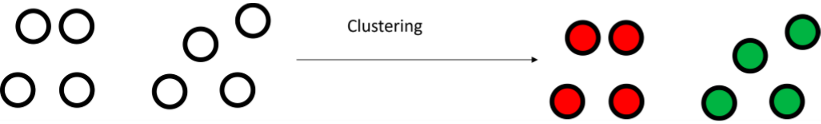
\includegraphics[scale=0.8]{Image/Clustering basics example.png}

There is a high intra\-cluster similarity and low inter\-cluster similarity.

\begin{itemize}
    \item Intra\-cluster cohesion (compactness): Cohesion measures how near the data points in a cluster are to the cluster centroid. 
    \item Inter\-cluster separation (isolation): Separation means that different cluster centroids should be far away from one another. 
\end{itemize}

\section{K-Means}
The K-Means algorithm partitions the given data into K clusters:
\begin{itemize}
    \item Each cluster has a cluster center (a.k.a centroid)
    \item K is manually specified by the user
\end{itemize}

\subsection{convergence (stopping) criteria}
\begin{itemize}
    \item no (or minimum) reassignment of data points to different clusters, or 
    \item no (or minimum) change of centroids or 
    \item minimum decrease in the sum of squared error (SSE)
\end{itemize}

Let $C_i$ be the $i$\-th cluster, and $\mu_i$ be the centroid of $C_i$ (the mean vector of all data points in $C_i$). If $x$ is the data point in the cluster and we are considering Euclidean distance:
\[\text{SSE}=\sum_{i=1}^{K}\sum_{x\in C_i}\text{disntace}(x,\mu_i)^2\]

\subsection{algorithm}
\begin{enumerate}
    \item Select K points as the initial centroids.
    \item repeat:
    \begin{enumerate}
        \item Form K clusters by assigning all points to the closest centroid.
        \item Recompute the centroid of each cluster.
    \end{enumerate}
    \item until fulfill the stopping condition
\end{enumerate}

\subsection{complexity}
No understanding for now. Check the slides

\subsection{Advantages}
\begin{itemize}
    \item Easy to understand and implement
    \item Efficient, if K and I are small, considered as a linear algorithm
    \item Scale to large data sets
    \item \textbf{Guarantee convergence}
    \item Clusters can be easily interpreted and even visualized.
    \item May produce tighter clusters than hierarchical clustering
\end{itemize}

\subsection{Disadvantages}
\begin{enumerate}
    \item K\-Means needs to \textbf{manually} set hyper\-parameter K.
    \begin{itemize}
        \item Sensitive to the hyper\-parameter of pre\-assigned number of clusters.
        \item Different K would lead to different clustering results.
    \end{itemize}
    So if K is too small, it will lead to insufficient partitioning. K too large will lead to over-partitioning.
    \item K\-Means algorithm is sensitive to outliers.
    \begin{itemize}
        \item Outliers are data points that are very far away from other data points.
        \item Outliers have a high influence since they can make SSE large, which will pull the center towards the outliers a lot.
    \end{itemize}
    \item K\-Means may not work well for data points with non\-globular shapes
    
    Since the cluster is based on Euclidean distance, the circular cluster is preferred and will be dominant:

    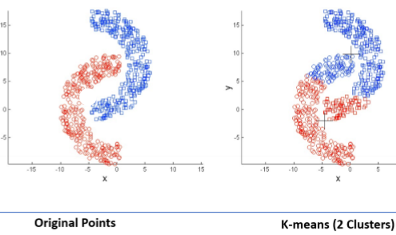
\includegraphics{Image/K means comparison unglobular shape.png}
\end{enumerate}

\section{Density-based clustering}

Different from K\-Menas:
\begin{itemize}
    \item Clusters are dense regions in the data space
    \item A cluster is defined as a maximal set of density-connected points 
    \item Noise points lie in regions of low-density
    \item Discover clusters of arbitrary shape and size.
\end{itemize}


\includegraphics[scale=0.8]{Image/DBSCAN V.S. K-Means.png}

\subsection{DBSCAN}
DBSCAN stands for Density\-based spatial clustering of applications with noise. 

Three parameters:
\begin{itemize}
    \item $\epsilon$: maximum radius of the neighborhood.
    \item $\epsilon-$Neighbor: data points within a radius of $\epsilon$ from a data point (including the point itself)
    \item \textit{MinPts}: minimum number of points required in a $\epsilon-$Neighbor.
\end{itemize}

Definition:
\begin{itemize}
    \item density is the number of points within a specified radius
    \item ``high density'' means data point's $\epsilon-$Neighbor contains at least MinPts data. 
\end{itemize}

Given $\epsilon$ and MinPts, categorize the data points into three:
\begin{enumerate}
    \item Core points: has more than or equal to MinPts within $\epsilon$. Should be at the interior of a cluster.
    \item Border point: has fewer than MinPts within $\epsilon$, but is in the neighborhood of a core point.
    \item Noise point or Outlier: any point that is neither a core point nor a border point. 
\end{enumerate}

As the name suggests, core points are in the center of a cluster, and border points form the border of the cluster and then enclose each cluster. 

\subsubsection{Density-reachable}
An object q is directly density-reachable from object p if p is a core object and q is in p's $\epsilon-$neighborhood. 

Note that it is not symmetric, reflexive or transitive. 

\subsection{algorithm}
\begin{enumerate}
    \item Label data points in core, border and noise
    \item Eliminate noise points
    \item For every \textbf{core points} p that has not been assigned to a cluster: Create a new cluster with the point p and all the points that are density\-connected to p. Then extend this to all core points in the same cluster till all no more directly reachable core points are available in the cluster.
    \item Assign border points to the cluster of the closest core point.
\end{enumerate}

\subsection{principles}
DBSCAN relies on a density\-based notion of the cluster: A cluster is defined as a maximal set of density\-connected points.
\begin{enumerate}
    \item Each cluster contains at least one core point.
    \item Given any two core points p and q, if N(p) contains q or N(q) contains p, then p and q are in the same cluster.
    \item A border point p is assigned arbitrarily to one of the clusters containing these core points. (Maybe choose the one with closer distance?)
    \item All noise points do not belong to any clusters.
\end{enumerate}

\subsection{Advantages}
\begin{itemize}
    \item DBSCAN can handle clusters of arbitrary shapes and sizes.
    \item Number of clusters is determined automatically, which is different from K\-Menas.
    \item Can separate clusters from noise, Robust to outliers.
    \item Also a very commonly used clustering algorithm.
\end{itemize}

\subsection{Disadvantages}
\begin{itemize}
    \item Sensitive to parameters: hard to determine the optimal parameters.
    \item Has problem identifying clusters of varying densities.
    \item DBSCAN may not work well in high\-dimensional data. (one dimension might dominate)
    \item Density estimation is kind of simplistic (e.g., does not create a real density function, but rather a graph of density-connected points)
\end{itemize}

\section{Principal Component Analysis (PCA)}
\subsection{The need for dimension reduction}
Samples in data sets might contain thousands of features. However, too many features not only cause computational problems but also might cause inaccuracy. 

\includegraphics*{Image/Classifier performance V.S. Dimensionality.jpg}

\subsubsection{Concept of dimensionality reduction}
Dimensionality reduction is the process in which we transform $X\in \mathbb{R}^D$ to $X'\in \mathbb{R}^d$. Here $X'$ represents $X$ when $d<<D$. 
\begin{itemize}
    \item $X'$ can be regarded as an approximation or abstraction of $X$
    \item it is expected to preserve the information of $X$ as much as possible while reducing the dimension. So it keeps only the feature with high variance. So other words, drop all the identical/repeated/common/similar features. 
\end{itemize}

Besides common patterns, correlated features can also be reduced. 
\begin{itemize}
    \item Consider some 2\-dimensional features $X_1,X_2$ for each dimension are two random variables.
    \item If the two random variables are \textbf{highly positive correlated}, we can observe these feature vectors are around a line spanned by vector $S$.
    \item In this way each feature vector can be \textbf{approximated} by $kS$.
    \item So we can use a 1\-dimensional vector with corresponding coefficient $k$ to represent a 2\-dimensional feature. 
\end{itemize}

\subsubsection{Projection}
Although feature spaces of raw data are always high dimensional. In many cases, feature vectors do not occupy the entire high\-dimensional feature space and most of them may lie around a low\-dimensional subspace of the ambient high\-dimensional space.

Thus, we can find a subspace of it to preserve the best representation of the original data. To represent, we orthogonally project a feature vector $X\in\mathbb{R}^D$ onto the subspace.

For example, the feature vector $\vec{X}$ is a $D\times 1$ vector. Then to represent with a lower dimension $d<<D$. We can use:
\[\vec{X}'=U\vec{X}\]
So $U$ is a $d\times D$ matrix that could lower the dimensionality and we need to find it. The same use can be extended to multiple data matrices.

Note that:
\begin{itemize}
    \item $U$ is an orthogonal matrix, meaning that elements $u_1,u_2,\ldots$ are all orthogonal to each other. 
    \item $UU^T X\neq X$ because projection will lose some information. 
\end{itemize}
 

The figure below illustrates an orthogonal projection of $X$ on the subspace spanned by $u_1,u_2$. 

\includegraphics*{Image/Projection to reduce dimensionality example.jpg}

\subsection{PCA algorithm}

One thing to note is that to correctly do PCA. It is important to normalize data. Otherwise, it is not going to produce the correct result. 

\subsubsection{Covariance}
Variance and Covariance measure the ``spread'' of a set of points around their center of mass (mean).
\begin{itemize}
    \item Variance measures the deviation from the mean for points in one dimension
    \item Covariance measures how much each of the dimensions varies from the mean with respect to each other. 
    \begin{itemize}
        \item Covariance is measured between two dimensions
        \item Covariance sees if there is a relation between two dimensions
        \item Covariance between one dimension is the variance
    \end{itemize}
\end{itemize}
We get positive Covariance when two dimensions are positively related, meaning increase and decrease at the same time. Negative Covariance would require the opposite behavior. 

We use it to find the relationships between two dimensions in high\-dimensional data sets:
\[q_{jk}=\frac{1}{N}(X_{ij}-E(X_j))(X_{ik}-E(X_k))\]
Note that the expected value is just the sample mean.

\subsubsection{Spectral theory}
PCA is related to eigenvalues. Review eigenvalue:
\[Av=\lambda v ,\forall A\in \mathbb{R}^{m\times n}\]
Any $\lambda, v$ pairs that satisfy the above relationship and are not zero are the eigenvalue and eigenvector. 

For symmetric $A, (m=n,A^T=A)$, it must have $n$ real eigenvalues and vectors. Here we replace $A$ with the data covariance matrix in PCA:

Give an example below:

    Want $X =  \begin{pmatrix}
        -1 & -1 & 0 & 2 & 0\\
        -2 & 0 & 0 & 1 & 1
    \end{pmatrix}$ to be reduced to 1 dimension where the first row is feature 0 and the second row is feature 1.

    \begin{enumerate}
        \item Normalize it so that each row has a mean of 0 (which is done already in the matrix)
        \item Find the Covariance matrix: (since the mean is 0, there is no subtraction)\[C = \frac{1}{N}XX^T=\frac{1}{5}\begin{pmatrix}
            -1 & -1 & 0 & 2 & 0\\
        -2 & 0 & 0 & 1 & 1
        \end{pmatrix}\begin{pmatrix}
            -1 & -2\\
            -1 & 0\\
            0 & 0\\
            2 & 1\\
            0 & 1
        \end{pmatrix} = \begin{pmatrix}
            \frac{6}{5} & \frac{4}{5}\\
            \frac{4}{5} & \frac{6}{5}
        \end{pmatrix}\]
        With that we can find eigenvalue and vector: \[\lambda_1 = 2, c_1=\begin{pmatrix}
            1\\1
        \end{pmatrix}, \lambda_2 = \frac{2}{5}, c_2=\begin{pmatrix}
            -1\\1
        \end{pmatrix}\]
        \item Now we standardize eigenvectors:\[\begin{pmatrix}
            c_1\\c_2
        \end{pmatrix}\implies P = \begin{pmatrix}
            \frac{1}{\sqrt{2}} & \frac{1}{\sqrt{2}}\\
            -\frac{1}{\sqrt{2}} & \frac{1}{\sqrt{2}}
        \end{pmatrix}\]

        \item Now we choose 1 eigenvector to lower it since we want a 1 D representation.
        \[Y = \begin{pmatrix}
            \frac{1}{\sqrt{2}} & \frac{1}{\sqrt{2}}
        \end{pmatrix} \begin{pmatrix}
            -1 & -1 & 0 & 2 & 0\\
        -2 & 0 & 0 & 1 & 1
        \end{pmatrix} = \begin{pmatrix}
            \frac{-3}{\sqrt{2}} & \frac{-1}{\sqrt{2}} & 0 & \frac{3}{\sqrt{2}} & \frac{-1}{\sqrt{2}}
        \end{pmatrix} \]
    \end{enumerate}
    Summarize the algorithm in words:
    \begin{enumerate}
        \item Find the mean of each feature
        \item Compute a $D\times D$ sample covariance.
        \item Find the first $d$ eigen vector of covariance. Note that $d<<D$ since it is the lower dimension you are aiming for
        \item Lastly, project it by timing the $d$ eigenvector matrix to the original data. 
    \end{enumerate}

\subsubsection{Optimization}
Choosing the larger eigenvalue would cause less loss of information. It can be found using the Variance percentage:
\[p_i = \frac{\lambda_i}{\sum\lambda_i}\]
So $\lambda_i>\lambda_j \implies$ $i^{th}$ eigenvector explains more variance.

\section{Nural Network basis}

Linear models need \textit{non-linearities} to be able to extend work to greater areas. Thus call for neural networks:
\subsection{Nonlinearities}
For linear regression, our loss function, for example, $(x,y)$ is:
\[L=\frac{1}{2}(y-\beta^T x-\beta_0)^2=\frac{1}{2}(y-f)^2\] 
where $f=\beta^T x+\beta_0$. Now consider $f=\beta^T h+\beta_0$:
\begin{itemize}
    \item If $h=Wx+b$, then it is still a linear model.
    \item We have to add a non-linear function $\Phi$ to it. Let $h=\Phi(Wx+b)$. But note that the last layer $f=\beta^T h+\beta_0$ is still linear.
\end{itemize}
This way, we can add as much information as we want while keeping the output linear.

\subsubsection{Activation (non\-linear) functions}
\begin{itemize}
    \item Sigmoid squashes real number to range between 0 and 1
    
    \includegraphics*{./Image/Sigmoid function.jpg}

    It is a non\-linear funciton:
    \begin{itemize}
        \item Countinuous which is easy to derivate. 
        \item Limited output range, easy to optimize, can be used as output layer.
    \end{itemize}

    When $x\to \pm \infty$, the gradient approaches 0, A.K.A \textbf{gradient vanishing}. It might terminate gradient descent undesirably. 

    Also, it is not centered at 0, making it slow in convergence.
    \item Tanh squashes real numbers to range between (-1,1)
    
    \includegraphics*{./Image/Tanh funciton.jpg}
    \[\text{Tanh}=2\times \text{Signmoid}-1=2\sigma(x)-1\]

    It is centered at 0, making it converge fast. However, it still experiences \textbf{gradient vanishing}, when $x\to \pm \infty$. 

    Also, the computational complexity is high since it involves too many exponentials. 

    \item ReLU (Rectified Linear Unit) is a step function $f(x)=\max(0,x)$.
    
    \includegraphics*{./Image/ReLU function.jpg}

    Compared to the previous two, it never experiences gradient disappearance since the gradient is never saturated and the convergence speed is fast. Also, no exponentials, so the calculation is fast and complexity is low.

    However, when $x<0$, the gradient is 0. Thus, the parameter is not updated, A.K.A \textbf{neuron death}. At the same time, the output mean value is greater than 0, which affects the convergence of the network. 
\end{itemize}

\subsection{Neruon meodel}
Here we model a neuron as a logistic unit:

\includegraphics*{./Image/Nueron Model.jpg}


\[Z=f_\theta(\vec{x})=\theta_1 x_1 + \theta_2 x_2 + \theta_3 x_3 + \theta_4\]
Here $\theta_4$ could be some constants introduced here. 

Now output is an activation function where $\vec{x}=[x_1,x_2,x_3]^T$, $\Theta=[\theta_1,\theta_2, \theta_3]^T$:
\[g_\Theta=\frac{1}{1+e^{-\Theta^T \vec{x}}}\]

The activation function exists so that we can get an answer of either 1 or 0. 

\subsection{Feed Forward}
\includegraphics*{./Image/Feed Forward Nonliearity.jpg}

The first layer is called the input, final layer is the output. Everything between the input and output are hidden layers as they cannot be seen.

Hidden layers are the ones to keep the training information by tuning the parameters. 

Here we can get value for layer 2 by:
\begin{itemize}
    \item $a_1^{(2)} = g(\Theta_{11}^{(1)}x_1+\Theta_{12}^{(1)}x_2+\Theta_{13}^{(1)}x_3)$
    \item $a_2^{(2)} = g(\Theta_{21}^{(1)}x_1+\Theta_{22}^{(1)}x_2+\Theta_{23}^{(1)}x_3)$
    \item $a_3^{(2)} = g(\Theta_{31}^{(1)}x_1+\Theta_{32}^{(1)}x_2+\Theta_{33}^{(1)}x_3)$
\end{itemize}

Here, $\Theta^{(1)}$ is the coefficient/weight from layer 1 to layer 2. g is the activation function. Note that g(x) is not linear!!!

Note that each calculation in a neural network only involves the data layer and the next layer. So a relationship can be extended to numerous layers without increasing the complexity of each calculation. 

\subsubsection{model complex function with non\-linearity}
Each neuron calculation can be seen as a step function with a corrected coefficient/weight that could be used to represent a piece of function.

Now if we cut a complex function infinitely small, then each small piece can be approximated using a step function with weights. This way, all functions can be modeled by a neural network. 

\subsection{Backpropagation}

A neural network consists of two components:
\begin{itemize}
    \item The network architecture, which defines layer numbers, neuron numbers and connections.
    \item The parameters, values of the connections and model weights.
\end{itemize}

\subsubsection{Before starting}
Before starting, we need to initialize the parameters:

In Practice, randomly initialize the parameters to small values, usually normally distributed around 0; $\mathcal{N}(0,0.1)$

\subsubsection{backpropagation algorithm}

\begin{enumerate}
    \item Input sample to the network and calculate the output (forward pass)
    \item Compare the output with the correct output to get the loss term.
    \item For all layers (backward pass from output layer, to hidden, to input)\begin{itemize}
        \item propagates the loss term back to the previous layer
        \item updates the weight between the two layers until the earliest hidden layer is reached 
    \end{itemize}
\end{enumerate}

Give a simple example:

\includegraphics*{./Image/Backpropagation example.jpg}

It is a simple illustration of $f(x,y,z)=(x+y)z$.

Note that:
\begin{align*}
    \frac{\partial q}{\partial x} & = 1 & \frac{\partial q}{\partial x} & = 1\\
    \frac{\partial f}{\partial q} & = z & \frac{\partial f}{\partial z} & = q
\end{align*}
\begin{align*}
    \frac{\partial f}{\partial x}& = \frac{\partial f}{\partial q} \frac{\partial q}{\partial x} = z\\
    \frac{\partial f}{\partial y}& = \frac{\partial f}{\partial q} \frac{\partial q}{\partial y} = z
\end{align*}

Because of the Chain Rule, we can build a gradient connection between the output and input via propagation. 

\subsection{Training and Validation}

General formulation:\begin{itemize}
    \item Given an input dataset $X=\{x_1,x_2,\ldots,x_n\}$ with corresponding label $Y=\{y_1,y_2,\ldots,y_m\}$
    \item Build a neural network with parameter $\Theta$
    \item Get prediction $\Hat{Y}=\{\hat{y_1},\hat{y_2},\ldots,\hat{y_m}\}$, where $\hat{y_i}=f(x_i,\Theta)$
    \item Total loss $\mathcal{L}=\sum_{i=1}^{n}l(y_i,\hat{y_i})$
\end{itemize}
\subsubsection{MSE}
We can use the mean square error as the loss:\begin{itemize}
    \item Mean square error (MSE) is the average squared difference between the estimated values and the actual value. MSE can be expressed by\[l_{MSE}=(y_i-\hat{y_i})^2=(y_i-f(c_i,\Theta))^2\]
    \item Further, we can compute the gradient of MSE by\[\frac{\partial l_{MSE}}{\partial \Theta}=-2(y_i-f(x_i,\Theta))\frac{\partial f(x_i,\Theta)}{\partial \Theta}\]
\end{itemize}
See the slides for an example
\subsection{Cross entropy error}
Cross entropy error (CE) is the cross\-entropy between two probability distributions over the same underlying set of events. \begin{itemize}
    \item CE can be expressed by \[l_{CE}=-y_i\log(\hat{y_i})=-y_i\log(f(x_i,\Theta))\]
    \item Further we can compute the gradient of CE by\[\frac{\partial l_{CE}}{\partial \Theta}=-\frac{y_i}{f(x_i,\Theta)}\frac{\partial (x_i,\Theta)}{\partial\Theta}\]
\end{itemize}
See the slides for an example
\subsubsection{Stochastic Gradient Descent (SGD)}

We use SGD be there is more than 1 optimal point or local minimum. We would aim for the global minimum:
\begin{align*}
    \theta_{t=1}&=\theta_t-\eta g(\theta_t)&\eta\text{ is the learning rate}\\
    g(\theta_t)&=\frac{1}{b}\sum_{i\in B_t}\nabla_\theta l(x_i;\theta_t)& b\text{ is the Batch size}
\end{align*}
\includegraphics*{./Image/SGD.jpg}
\subsubsection{Training}
\begin{itemize}
    \item One Epoch is completed when a complete data set is cycled forward and backward through the neural network.
    \item Batch size is a parameter that defines the number of samples to work through before updating the neural network weights.
    \item Iterations are the number of batches needed to complete on epoch
\end{itemize}
\subsubsection{Learning rate decay}
We should reduce the learning rate as we complete more Epoch. Since we do not want oscillations when getting to the correct gradient. There are lots of ways to decay:\begin{enumerate}
    \item Step decay: reduce the rate at a few fixed points, making it as stairs.
    \item Linear decay: linearly decay proportional to the number of Epoch
    \item Cosine decay
    \item Inverse square root decay
\end{enumerate}

\section{NN advance}
There are lots of variants if neural network:\begin{itemize}
    \item Convolutional Neural Networks (CNN): Popular for Image Data, directly applicable for 2D representations
    \item Recurrent Neural Networks (RNN): Contains self-loop, Good for Sequential data.
    \item Generative Adversarial Network (GAN):
    \item Transformer: 
    \item Graph Neural Networks (GNN): deal with graph inputs. 
\end{itemize}
\subsection{AutoEncoder(AE)}
Here are some important aspects for AE:\begin{itemize}
    \item Unsupervised: No labels used, discovers useful features of the input. 
    \item Compression: Code reduces the dimension of data
    \item Lossy: input won't be reconstructed exactly
    \item Trained: The compression algorithm is learned for specific data
\end{itemize}

\section{Ok! Neural Network is too hard, comeback and fill it when my math improves}












\end{document}

An example of Boosting is ``AdaBoost''

\begin{enumerate}
    \item Initialize the observation weight $w_i = \frac{1}{N}, \forall i \in \mathbb{N}, i \le N$. Here there are $N$ data.
    \item $\forall m  \in \mathbb{N}, m \le M$
    \begin{enumerate}
        \item Fit a classifier $G_m(x)$ to the training data using $w_i$
        \item Compute error: $\text{err}_m = 
    \end{enumerate}
\end{enumerate}